\documentclass{article}
\usepackage{titling}
\usepackage{lipsum}
\usepackage{amsmath}
\usepackage{listings}
\usepackage{graphicx}



\begin{document}
\noindent
\begin{minipage}[t]{0.6\textwidth}
    \begin{flushleft}
        \LARGE\textbf{Math 343 - Homework 1} \\
        \vspace{6pt} % add 6pt of vertical space
        \hrule width 10cm
        \vspace{12pt}
        \large\textbf{Preston Duffield} \\
        \large Western Washington University \\
        \today
        \vspace{24pt}
    \end{flushleft}
\end{minipage}


\section*{Question 1}

\subsection*{a)}
\subsection*{b)}
\subsection*{c)}
\subsection*{d)}

\section*{Question 2}

First we note that,
% t = (y-bar/mu_0)/S/root(n) is approximately N(0,1).
\begin{equation*}
    t = \frac{\bar{X} - \mu_0}{S/\sqrt{n}} \sim N(0,1)
    \end{equation*}
\begin{flushleft}
Then we can derive that,
    \end{flushleft}
    
    % As long as the sample size is sufficiently large and the population is normal or the sample size is very large, the statement is generally true by the Central Limit Theorem.
\begin{align*}
    1 - \alpha &= P(-t_{\alpha,n-1} \leq \frac{\bar{X} - \mu_0}{S/\sqrt{n}} \leq t_{\alpha,n-1}) \\
                &= P(-t_{\alpha,n-1} \frac{S}{\sqrt{n}} \leq \bar{X} - \mu_0 \leq t_{\alpha,n-1} \frac{S}{\sqrt{n}}) \\
                &= P(-\bar{X} - t_{\alpha,n-1} \frac{S}{\sqrt{n}} \leq -\mu_0 \leq -\bar{X} + t_{\alpha,n-1} \frac{S}{\sqrt{n}}) \\
                &= P(\bar{X} + t_{\alpha,n-1} \frac{S}{\sqrt{n}} \geq \mu_0 \geq \bar{X} - t_{\alpha,n-1} \frac{S}{\sqrt{n}}) \\
                &= P(\bar{X} - t_{\alpha,n-1} \frac{S}{\sqrt{n}} \leq \mu_0 \leq \bar{X} + t_{\alpha,n-1} \frac{S}{\sqrt{n}})
    \end{align*}

Therefore, the confidence interval for one population mean $\mu$ in the case
where the population variance $\sigma ^{2}$ is unknown can be described as

\begin{align*}
    \bar{X} \pm t_{\alpha,n-1}\frac{S}{\sqrt{n}}
\end{align*}

\section*{Question 3}
The P-value can be obtained in R using the following code, where $t_0$ varies.
\begin{lstlisting}[language=R, caption=Calculating the P-value for a $t_0$ value, basicstyle=\small]
    # Define the t_0 value, degrees of freedom, and tail of the distribution
    t_0 <- 2.48
    df <- 10
    tail <- 2
    
    # Calculate the P-value using the "pt" function
    p_val <- pt(t_0, df, tail)
    
    # Print the P-value
    print(p_val)
    \end{lstlisting}

\subsection*{a)}
When $t_0 = 2.48$, the P-value is $0.637$.
\subsection*{b)}
When $t_0 = 3.55$, the P-value is $0.869$.
\subsection*{c)}
When $t_0 = 2.00$, the P-value is $0.478$.

\section*{Question 4}

\subsection*{a)}

\begin{figure}[h]
    \centering
    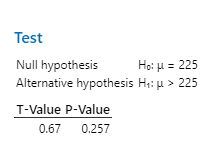
\includegraphics[width=0.5\textwidth]{./hw_1/images/4_b.png}
    \caption{The output of the 1-sample t test from Minitab.}
    \label{fig:4_a}
  \end{figure}

\subsection*{b/c)}
Since the p-value (0.257)
is greater than the significance level (0.05),
we fail to reject the null hypothesis. That is,
there is not have enough statistical evidence to support that the mean repair
time exceeds 225 hours.
\subsection*{d)}
\begin{figure}[h]
    \centering
    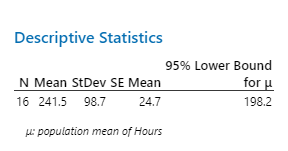
\includegraphics[width=0.5\textwidth]{./hw_1/images/4_a.png}
    \caption{The Descriptive Statistics of the 1-sample t test from Minitab.}
    \label{fig:4_b}
  \end{figure}



\section*{Question 5}

\subsection*{a)}
\subsection*{b)}
\subsection*{c)}
\subsection*{d)}
\subsection*{e)}

\section*{Question 6}

\section*{Question 7}
\end{document}
